\documentclass{article}

% \usepackage[english]{babel}
\usepackage[brazilian]{babel}
\usepackage[letterpaper,top=2cm,bottom=2cm,left=3cm,right=3cm,marginparwidth=1.75cm]{geometry}

% Useful packages
\usepackage{amsmath}
\usepackage{graphicx}
% \usepackage[colorlinks=true,linkcolor=blue]{hyperref}
\usepackage{hyperref}
\usepackage{listings}
\usepackage[figure,table,lstlisting]{totalcount}
\usepackage{tcolorbox}
\usepackage{listings}
\usepackage{xcolor}

\hypersetup{
    colorlinks=true,
    linkcolor=black,
    filecolor=magenta,      
    urlcolor=cyan,
    pdftitle={Overleaf Example},
    pdfpagemode=FullScreen,
    }

\definecolor{verde}{rgb}{0.25,0.5,0.35}
\definecolor{jpurple}{rgb}{0.5,0,0.35}

\lstset{
  language=C++,
  basicstyle=\ttfamily\small,
  keywordstyle=\color{jpurple}\bfseries,
  stringstyle=\color{red},
  commentstyle=\color{verde},
  morecomment=[s][\color{blue}]{/**}{*/},
  extendedchars=true,
  showspaces=false,
  showstringspaces=false,
  numbers=left,
  numberstyle=\tiny,
  breaklines=true,
  backgroundcolor=\color{cyan!10},
  breakautoindent=true,
  captionpos=b,
  xleftmargin=0pt,
  tabsize=4
}

\renewcommand{\lstlistingname}{Código}
\renewcommand{\lstlistlistingname}{Lista de Códigos Fonte}

\newcommand\conditionalLoF{%
    \iftotalfigures
        \listoffigures
    \fi}
\newcommand\conditionalLoT{%
    \iftotaltables
        \listoftables
    \fi}
\newcommand\conditionalLoL{%
    \iftotallstlistings
        \lstlistoflistings
    \fi}

\newcommand{\DESCRICAO}[1]{
    % set flexible interword space
    \setlength{\spaceskip}{0.5em plus 1em minus 0.1em}%
    % add some space with not as much flexibility, but only
    % if some space precedes
    \ifdim\lastskip>0pt \hspace{0.5em plus 0.5em minus 0.1em}\fi
    \texttt{\textbf{\color{red}#1}}
}

\newcommand{\CAPA}[6]{
    % 1) Título
    % 2)
    % 3)
    % 4)
    \begin{titlepage}
    	
    	  \vfill
    	
    	  \begin{center}
    	    \begin{large}
    	      Universidade Federal de Ouro Preto - UFOP
    	    \end{large}
    	  \end{center}
    	
    	  \begin{center}
    	    \begin{large}
    	      Instituto de Ciências Exatas e Biológicas - ICEB
    	    \end{large}
    	  \end{center}
    	
    	  \begin{center}
    	    \begin{large}
    	      Departamento de Computação - DECOM
    	    \end{large}
    	  \end{center}
          
          \begin{center}
    	    \begin{large}
              Ciência da Computação
    	    \end{large}
    	  \end{center}
    	  
    	  \vfill
          \vfill
    	
    	  \begin{center}
    	    \begin{Huge}
    	      #1\\
    	    \end{Huge}
    	    \begin{Large}
              #2\\
    	    \end{Large}
    	  \end{center}
    	  
    	  \vfill
    	  
    	  \begin{center}
    	    \begin{large}
              #3
    	    \end{large}
    	  \end{center}

        \begin{center}
    	    \begin{large}
              #4
    	    \end{large}
    	  \end{center}

        \begin{center}
    	    \begin{large}
              #5
    	    \end{large}
    	  \end{center}
    	
    	  \begin{center}
    	    \begin{large}
    	      Professor: #6
    	    \end{large}
    	  \end{center}
    	
    	  \vfill
          \vfill
    	
    	  \begin{center}
    	    \begin{large}
    	      Ouro Preto \\
    	      \today \\
    	    \end{large}
    	  \end{center}    
    
    
    \clearpage
    \newpage

    \tableofcontents
    \conditionalLoF
    \conditionalLoT
    \conditionalLoL
	
    % \thispagestyle{empty}
    % \tableofcontents
    % \newpage
    % \thispagestyle{empty}
    
    % \listoffigures
    
    % \lstlistoflistings
    % \newpage
    % \thispagestyle{empty}
    \end{titlepage}
}

\begin{document}

\CAPA{Trabalho Prático II}{BCC266 - Organização de Computadores}{Vitor Oliveira Diniz}{Maria Luiza Aragão}{Jéssica Machado}{Pedro Silva}



\section{Introdução}
A memória cache funciona como uma biblioteca de acesso rápido que existe dentro de computadores e dispositivos móveis. Ela tem o objetivo de guardar dados, informações e processos temporários acessados com frequência e assim agilizar o processo de uso no momento em que são requisitados pelo usuário.

\subsection{Especificações do problema}

Para este trabalho prático, deveríamos, a partir dos caches 1 e 2 que foram disponibilizados pelo professor, implementar a memória cache 3 e fazer a movimentação de dados entre os diferentes tipos de cache.
\subsection{Considerações Iniciais}
Algumas ferramentas foram utilizadas durante a criação deste projeto:

\begin{itemize}
  \item Ambiente de desenvolvimento do código fonte: Visual Studio Code.
  \item Linguagem utilizada: C.
  \item Ambiente de desenvolvimento da documentação: Visual Studio Code \LaTeX Workshop.
\end{itemize}

\subsection{Ferramentas utilizadas}
Algumas ferramentas foram utilizadas para testar a implementação, como:

\begin{itemize}
    \item[-] \textit{CLANG}: ferramentas de análise estática do código.
    \item[-] \textit{Valgrind}: ferramentas de análise dinâmica do código.
\end{itemize}

\subsection{Especificações da máquina}
A máquina onde o desenvolvimento e os testes foram realizados possui a seguinte configuração:

\begin{itemize}
    \item[-] Processador: Ryzen 7-5800H.
    \item[-] Memória RAM: 16 Gb.
    \item[-] Sistema Operacional: Arch Linux x86\_64.
\end{itemize}


\subsection{Instruções de compilação e execução}

Para a compilação do projeto, basta digitar:

\begin{tcolorbox}[title=Compilando o projeto,width=\linewidth]
    gcc main.c -c -Wall \newline
    gcc mmu.c -c -Wall \newline
    gcc memory.c -c -Wall\newline
    gcc instruction.c -c -Wall\newline
    gcc cpu.c -c -Wallnewline
    gcc generator.c -c -Wall\newline
    gcc main.o mmu.o memory.o instruction.o cpu.o generator.o -o exe -g
\end{tcolorbox}

Usou-se para a compilação as seguintes opções:

\begin{itemize}
    \item [-] \emph{-Wall}: para mostrar todos os possível \emph{warnings} do código.
    \item [-] \emph{-c}: Para compilar o arquivo sem linkar os arquivos para obtermos um arquivo do tipo objeto.
    \item [-] \emph{-o}: Compilar para um arquivo do tipo output $($saída$)$.
\end{itemize}

Para a execução do programa basta digitar um dos exemplos:
\begin{tcolorbox}[title=,width=\linewidth]
    ./exe random [TAMANHO DA RAM] [L1] [L2] [L3] \newline


\end{tcolorbox}


\clearpage



\section{Desenvolvimento}

Seguindo as boas práticas de programação, implementamos uma memória cache particionada em linhas e simulamos o mapeamento associativo para a troca das mesmas com a memória RAM. Usamos as políticas LFU (Last Frequently Used) e LRU (Last Recently Used) como métodos de otimização.



\subsection{Operações}

A seguir entraremos em detalhe sobre as principais funções utilizadas no programa e as coisas que implementamos.

\subsubsection{Médodos de mapeamento}

Define o tipo de método que vai ser usado para a saída dos resultados.

\begin{lstlisting}[caption={Definição do tipo de método},label={lst:cod1},language=C]

    // 1 MAPEAMENTO DIRETO
    // 2  LRU (Least Recently Used)
    // 3  LFU (Least Frequently Used)

    #define SUBSTITUTION_METHOD 3
    
\end{lstlisting}

\subsubsection{TAD Machine}

Adicionamos cache L3, o hitL3 (que conta quantas vezes processador achou o dado na cache) e o missL3 (que conta quantas vezes o processador precisou buscar o dado na memória ou até no disco).

\begin{lstlisting}[caption={TAD Machine},label={lst:cod2},language=C]

    typedef struct {
        Instruction* instructions;
        RAM ram;
        Cache l1; // cache L1
        Cache l2; // cache L2
        Cache l3; // cache L3
        int hitL1, hitL2, hitL3, hitRAM;
        int missL1, missL2, missL3;
        int totalCost;
        } Machine;

    \end{lstlisting}

\subsubsection{run}

Inicializa o contador PC com valor 0 e, enquanto o opcode de machine-$>$instructions[PC] for diferente de -1 (condição de parada), printamos a quantidade de vezes que o processador achou (hit) o dado na L1, L2, L3 e RAM, a quantidade de vezes que o processador precisou buscar o dado na memória ou até no disco (miss), e o custo total.

\begin{lstlisting}[caption={Funçao run},label={lst:cod3},language=C]
    void run(Machine* machine) {    
        int PC = 0; // Program Counter
        while(machine->instructions[PC].opcode != -1) {
            executeInstruction(machine, PC++);
            printf("\tL1:(%6d, %6d) | L2:(%6d, %6d) | L3:(%6d, %6d) | RAM:(%6d) | COST: %d\n", 
                machine->hitL1, machine->missL1, 
                machine->hitL2, machine->missL2,
                machine->hitL3, machine->missL3,
                machine->hitRAM,
                machine->totalCost);
        }
}
    
    
\end{lstlisting}

\subsubsection{printMemories}

Printa as informações da RAM, se está atualizado é a cor verde e, se não, cor vermelha.

\begin{lstlisting}[caption={Função printMemories},label={lst:cod4},language=C]
    void printMemories(Machine* machine) {
        printf("\x1b[0;30;47m     ");
        printc("RAM", WORDS_SIZE * 8 - 1);
        printc("Cache L3", WORDS_SIZE * 8 + 6);
        printc("Cache L2", WORDS_SIZE * 8 + 6);
        printc("Cache L1", WORDS_SIZE * 8 + 6);
        printf("\x1b[0m\n");
    
    
    
        for (int i=0;i<machine->ram.size;i++) {
            printf("\x1b[0;30;47m%5d|\x1b[0m", i);
            for (int j=0;j<WORDS_SIZE;j++)
                printf(" %5d |", machine->ram.blocks[i].words[j]);
    
            if (i < machine->l3.size) {
                printf("|");
                printcolored(machine->l3.lines[i].tag, machine->l3.lines[i].updated);
                for (int j=0;j<WORDS_SIZE;j++)
                        printf(" %5d |", machine->l3.lines[i].block.words[j]);
    
                if (i < machine->l2.size) {
                    printf("|");
                    printcolored(machine->l2.lines[i].tag, machine->l2.lines[i].updated);
                    for (int j=0;j<WORDS_SIZE;j++)
                        printf(" %5d |", machine->l2.lines[i].block.words[j]);
                    if (i < machine->l1.size) {
                        printf("|");
                        printcolored(machine->l1.lines[i].tag, machine->l1.lines[i].updated);
                        for (int j=0;j<WORDS_SIZE;j++)
                            printf(" %5d |", machine->l1.lines[i].block.words[j]);
                    }
                }
            }
            printf("\n");
        }
    }
    

\end{lstlisting}
\clearpage
\subsubsection{startCache}

Aloca dinamicamente as linhas e inicia a cache com o valor inválido (-1).

\begin{lstlisting}[caption={startCache},label={lst:cod6},language=C]
    // ALOCA DINAMICAMENTE A CACHE COM UM TAMANHO ESPECIFICO
    void startCache(Cache* cache, int size) {
        cache->lines = (Line*) malloc(sizeof(Line) * size);
        cache->size = size;
    
        // INICIA A CACHE COM UM VALOR INVALIDO -1
        for (int i=0;i<size;i++){
            cache->lines[i].tag = INVALID_ADD;
            cache->lines[i].timeOnCache = 0;
            cache->lines[i].timesUsed = 0;
        }
    }

\end{lstlisting}

\subsubsection{TAD Line}

Adicionamos as variáveis timesUsed, do tipo inteiro, para contar quantas vezes a variável passada para a cache foi usada, e a timeOnCache o tempo que informação ficou sem ser acessada.

\begin{lstlisting}[caption={TAD Line},label={lst:cod6},language=C]

    typedef struct {
        MemoryBlock block; // BLOCO DE MEMORIA, QUE CONTEM 1 VETOR DE PALAVRAS, O BLOCO REPRESENTA CACHE L1 L2 L3 E RAM
        int tag; /* Address of the block in memory RAM */
        bool updated;
        int cost; // custo de acesso a CACHE/RAM
        int cacheHit;
        int timesUsed;
        int timeOnCache;
    } Line;

\end{lstlisting}

\subsubsection{memoryCacheMapping}

Essa função é responsável por checar qual tipo de mapeamento estamos utilizando e, dependendo do mapeamento,
iremos aplicar uma política diferente. No caso do mapeamento direto, retornamos o possível endeeço da cache e a verificação
de sua existência é feita no MMUSearchOnMemorys. No caso da LRU, percorremos o vetor sempre checando qual endereço está a mais tempo na cache
e salvando seu índice, caso encontremos o endereço que procuramos retornamos seu índice, se a substituição vai acontecer ou não depende do MMUSearchOnMemorys.
No LFU acontece a mesma coisa que o LRU, apenas mudando a condição de checagem para o bloco menos usado.

\begin{lstlisting}[caption={Função memoryCacheMapping},label={lst:cod6},language=C]

    int memoryCacheMapping(int address, Cache* cache) {

    int index = 0;

    switch(SUBSTITUTION_METHOD){
        //DIRECT MAPPING
        case 1:
            return address % cache->size;
            break;
        //LRU METHOD (Least Recently Used)
        case 2:
            cache->lines[0].timeOnCache++;
            for( int i = 0; i < cache->size; i++){
                
                cache->lines[i].timeOnCache++;

                if(cache->lines[i].timeOnCache > cache->lines[index].timeOnCache)
                    index = i;
                
                if(cache->lines[i].tag == address)
                    return i;

            }
            return index;
            break;

        //LFU METHOD (Least Frequently Used)
        case 3:
            for( int i = 0; i < cache->size; i++){
                if(cache->lines[i].timesUsed < cache->lines[index].timesUsed)
                    index = i;

                if(cache->lines[i].tag == address)
                    return i;
            }

            return index;
            break;
    }

    return address % cache->size;
}

\end{lstlisting}

\subsubsection{updateMachineInfos}

Modificamos os valores de hit e miss da cache l3, contamos quantas a linha foi usada e o custo.

\begin{lstlisting}[caption={Função updateMachineInfos},label={lst:cod6},language=C]

    void updateMachineInfos(Machine* machine, Line* line) {


        switch (line->cacheHit) {
            case 1:
                machine->hitL1 += 1;
                break;

            case 2:
                machine->hitL2 += 1;
                machine->missL1 += 1;
                break;
            
            case 3:
                machine->hitL3 += 1;
                machine->missL1 += 1;
                machine->missL2 += 1;
                break;
            
            case 4:
                machine->hitRAM += 1;
                machine->missL1 += 1;
                machine->missL2 += 1;
                machine->missL3 += 1;
                break;
        }

        line->timeOnCache = 0;
        line->timesUsed++;

        machine->totalCost += line->cost;
    }   

\end{lstlisting}
\clearpage

\subsubsection{MMUSearchOnMemorys}

Inicialmente, essa função pega a possível posição do bloco que queremos na CACHE e conferimos se o
que queremos está realmente na RAM. Se estiver, atualizamos o cache hit referente aonde ele se encontra,
o custo de acesso da memória, a nossa máquina e retornamos a linha que o endereço se encontra. Se não encontrarmos o 
endereço na cache, fazemos as movimentações necessárias entre as memórias, levando em consideração o mapeamento
escolhido e, caso precise, levamos o endereço da cache para RAM.


\begin{lstlisting}[caption={Função MMUSearchOnMemorys},label={lst:cod6},language=C]

    Line* MMUSearchOnMemorys(Address add, Machine* machine) {
    // Strategy => write back
    
    // Direct memory map
    int l1pos = memoryCacheMapping(add.block, &machine->l1);
    int l2pos = memoryCacheMapping(add.block, &machine->l2);
    int l3pos = memoryCacheMapping(add.block, &machine->l3);


    Line* cache1 = machine->l1.lines;
    Line* cache2 = machine->l2.lines;
    Line* cache3 = machine->l3.lines;

    // adicionar linha da L3
    MemoryBlock* RAM = machine->ram.blocks;

    if (cache1[l1pos].tag == add.block) { 
        /* Block is in memory cache L1 */
        // ESTA FALTANDO TAG E UPDATED
        cache1[l1pos].cost = COST_ACCESS_L1;
        cache1[l1pos].cacheHit = 1;
    } else if (cache2[l2pos].tag == add.block) { 
        /* Block is in memory cache L2 */
        cache2[l2pos].tag = add.block;
        cache2[l2pos].updated = false;
        cache2[l2pos].cost = COST_ACCESS_L1 + COST_ACCESS_L2;
        cache2[l2pos].cacheHit = 2;
        updateMachineInfos(machine, &(cache2[l2pos]));

        return &(cache2[l2pos]);
    } else if (cache3[l3pos].tag == add.block){
        /* Block is in memory cache L3 */
        cache3[l3pos].tag = add.block;
        cache3[l3pos].updated = false;
        cache3[l3pos].cost = COST_ACCESS_L1 + COST_ACCESS_L2 + COST_ACCESS_L3;
        cache3[l3pos].cacheHit = 3;

        updateMachineInfos(machine, &(cache3[l3pos]));
        return &(cache3[l3pos]);

    } else { 
        /* Block only in memory RAM, need to bring it to cache and manipulate the blocks */
        //fazer o mapeamento para decidir quem tirar da ram.
        l2pos = memoryCacheMapping(cache1[l1pos].tag, &machine->l2); /* Need to check the position of the block that will leave the L1 */
        l3pos = memoryCacheMapping(cache2[l2pos].tag, &machine->l3); /* Need to check the position of the block that will leave the L1 */

        
        if (!canOnlyReplaceBlock(cache1[l1pos])) { 
            /* The block on cache L1 cannot only be replaced, the memories must be updated */
            if (!canOnlyReplaceBlock(cache2[l2pos])){
                /* The block on cache L2 cannot only be replaced, the memories must be updated */
                if(!canOnlyReplaceBlock(cache3[l3pos])){
                    /* The block on cache L2 cannot only be replaced, the memories must be updated */
                    RAM[cache3[l3pos].tag] = cache3[l3pos].block;
                }
                cache3[l3pos] = cache2[l2pos];
                cache3[l3pos].timeOnCache = 0;


            }

            cache2[l2pos] = cache1[l1pos];
            cache2[l2pos].timeOnCache = 0;

        }

        
        cache1[l1pos].block = RAM[add.block];
        cache1[l1pos].tag = add.block;
        cache1[l1pos].updated = false;
        cache1[l1pos].cost = COST_ACCESS_L1 + COST_ACCESS_L2 + COST_ACCESS_L3 + COST_ACCESS_RAM;

        //se passa da l1 para a l2 eu deveria zerar ?
        cache1[l1pos].cacheHit = 4;
        cache1[l1pos].timeOnCache = 0;


    }
    updateMachineInfos(machine, &(cache1[l1pos]));
    return &(cache1[l1pos]);
}

\end{lstlisting}

\clearpage

\subsection{Função Main}

Na função main adicionamos mais um espaço a memoriesSize para a l3.

\begin{lstlisting}[caption={Main},label={lst:cod6},language=C]
    int main(int argc, char**argv) {

        srand(1507);   // Inicializacao da semente para os numeros aleatorios.

        if (argc != 6) {
            printf("Numero de argumentos invalidos! Sao 6.\n");
            printf("Linha de execucao: ./exe TIPO_INSTRUCAO [TAMANHO_RAM|ARQUIVO_DE_INSTRUCOES] TAMANHO_L1 TAMANHO_L2 TAMANHO_L3\n");
            printf("\tExemplo 1 de execucao: ./exe random 10 2 4 6\n");
            printf("\tExemplo 2 de execucao: ./exe file arquivo_de_instrucoes.txt\n");
            return 0;
        }

        int memoriesSize[4];
        Machine machine;
        Instruction *instructions;

        memoriesSize[1] = atoi(argv[3]);
        memoriesSize[2] = atoi(argv[4]);
        memoriesSize[3] = atoi(argv[5]);


        if (strcmp(argv[1], "random") == 0) {
            memoriesSize[0] = atoi(argv[2]);
            instructions = generateRandomInstructions(memoriesSize[0]);
        } else if (strcmp(argv[1], "file") == 0) {
            instructions = readInstructions(argv[2], memoriesSize);
        } 
        else {
            printf("Invalid option.\n");
            return 0;
        }
        
        printf("Starting machine...\n");
        start(&machine, instructions, memoriesSize);
        if (memoriesSize[0] < 10)
            printMemories(&machine);
        run(&machine);
        if (memoriesSize[0] < 10)
            printMemories(&machine);
        stop(&machine);
        printf("Stopping machine...\n");
        return 0;
    }
\end{lstlisting}
\clearpage


\section{Impressões Gerais}
Primeiramente, nos reunimos no discord para a leitura e compreensão do documento e arquivos disponibilizados para a realização do trabalho.
O código disponibilizado estava bem legível o que facilitou um pouco, mas nas aulas faltaram demonstrações/implementações dos métodos de mapeamento. 
Também encontramos dificuldade de entender a tabela que estava no PDF, porém, esse problema foi resolvido posteriormente com certa facilidade. Um dos pontos positivos foi quando o professor disponibilizou tempo de aula para sanar nossas dúvidas.
Para a documentação utilizamos o \LaTeX, o que não nos trouxe dificuldade devido ao prévio conhecimento adquirido com trabalhos anteriores. 
Descobrimos uma extensão bastante útil do VS Code: o Live Share, que nos permitiu editar o código simultaneamente.
\clearpage
\section{Análise}

Após a análise da parte já disponibilizada do código, identificamos implementações de funções que já havíamos aplicado no trabalho anterior, como a soma, subtração e movimentação de dados.
Tendo isso em vista, construímos o raciocínio da aplicação da cache L3, seguindo a mesma linha de pensamento das memórias já implementadas anteriormente. 
Partimos então para o mapeamento associativo e as movimentações de troca, ponderando sobre as políticas LFU (Last Frequently Used) e LRU (Last Recently Used).

\subsection{Análise de Complexidade}
Na função memoryCacheMapping, a sua complexidade vai depender do método de mapeamento escolhido. Para o mapeamento direto, 
como não percorremos o vetor, já que a posição na cache depende unicamente do final de seu endereço, 
sua complexidade será $\mathcal{O}(1)$. \\

Na política LRU, na função memoryCacheMapping, percorremos o vetor para encontrar o bloco que está a mais tempo sem ser utilizado, por isso 
teremos uma complexidade de $\mathcal{O}(n)$. \\

Na política LFU, na memoryCacheMapping, também percorremos o vetor para encontrar o bloco que está a mais tempo sem ser utilizado, por isso 
teremos uma complexidade de $\mathcal{O}(n)$.
\clearpage

\begin{figure}
    \centering
    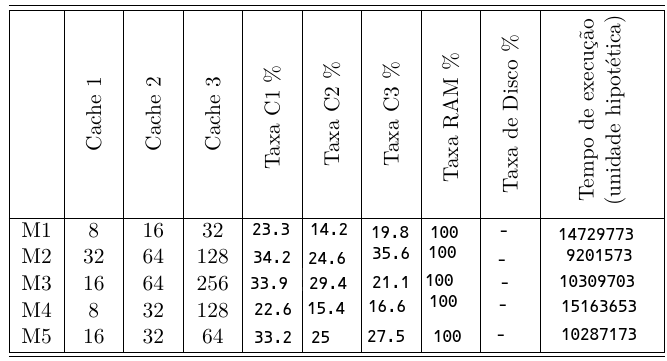
\includegraphics[width=0.8\textwidth]{mapeamento.png}
    \caption{Mapeamento Direto}
    \label{fig:Tabela 1}
\end{figure}

\begin{figure}
    \centering
    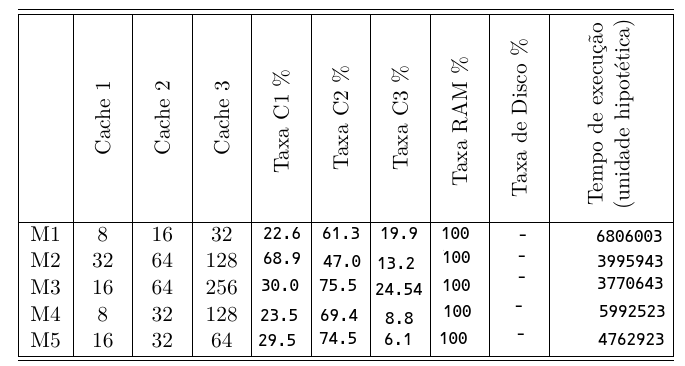
\includegraphics[width=0.8\textwidth]{lru.png}
    \caption{LRU}
    \label{fig:Tabela 2}
\end{figure}

\begin{figure}
    \centering
    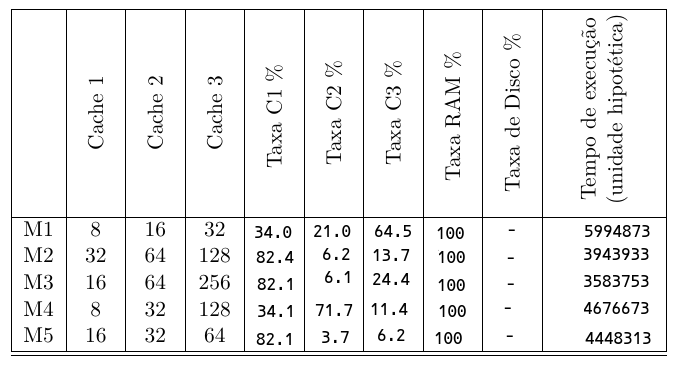
\includegraphics[width=0.8\textwidth]{lfu.png}
    \caption{LFU}
    \label{fig:Tabela 3}
\end{figure}

\clearpage
\section{Conclusão}
Com este trabalho, aprendemos sobre a memória CACHE e movimentação de dados entre diferentes tipos de cache, dependendo do
tipo de mapeamento usado.
Entre as políticas de mapeamento, o mapeamento direto é, sem dúvidas, o pior método de todos. Já entre o LFU e LRU,
os resultados adquiridos na comparação entre o cache hit e cache miss foram semelhantes.
Uma das dificuldades encontradas foi a falta de uma saída teste para efeitos de comparação para que a gente pudesse ver 
se a saída do nosso programa está correta. Dito isso, achamos a dinâmica do trabalho excelente e bem didática possamos aprender de um jeito palpável esses conceitos.

\end{document}